\section{Muhammad Reza Syachrani - 1174084}
\subsection{Teori}
\begin{enumerate}

	\item Jelaskan kenapa kata-kata harus di vektorisasi, dan gambar ilustrasi
	\hfill\\
Kata-kata divektorisasi agar mechine learning dapat memprosesnya karena mechine learning tidak dapat membaca data text langsung sehingga perlu dilakukan vektorisasi untuk mengukur nilai dari suatu kata sehingga dapat mengetahui bobot dari setiap kata agar dapat dibaca dan melakukan prediksi.
\begin{figure}[H]
    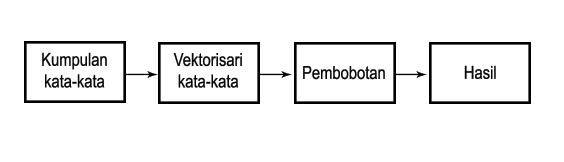
\includegraphics[width=12cm]{figures/1174084/5/teori1.png}
    \centering
    \caption{Teori 1}
\end{figure}

\item Jelaskan mengapa dimensi dari vektor dataset google bisa sampai 300. Dilengkapidengan ilustrasi atau gambar.
	\hfill\\
	Dimensi dataset dari google bisa mencapai 300 karena dimensi dari vektor tersebut digunakan untuk membandingkan bobot dari setiap kata, misalkan terdapat kata dog dan cat pada dataset google tersebut setiap kata tersebut di buat dimensi vektor 300 untuk kata dog dan 300 dimensi vektor juga untuk kata cat kemudian kata tersebt di bandingkan bobot kesamaan katanya maka akan muncul akurasi sekitar 70 persen kesamaan bobot dikarenakan kata dog dan cat sama sama di gunakan untuk hewan priharaan.

\begin{figure}[H]
    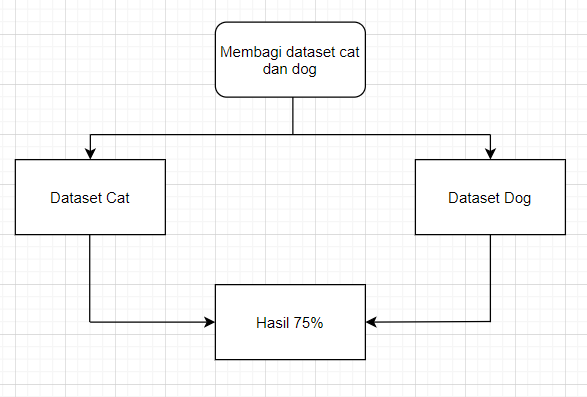
\includegraphics[width=12cm]{figures/1174084/5/teori2.png}
    \centering
    \caption{Teori 2}
\end{figure}

\item Jelaskan konsep vektorisasi untuk kata.dilengkapi dengan ilustrasi atau gambar.
	\hfill\\
	Vektorisasi untuk kata untuk mengetahui kata tengah dari suatau kalimat atau kata utama atau objek utama pada suatau kalimat contoh ( Jangan lupa subscribe channel saya ya sekian terimamakasih ) kata tengah tersebut merupakan channel yang memiliki bobot sebagai kata tengah dari suatu kalimat atau bobot sebagai objek dari suatu kalimat. hal ini sangat berkaitan dengan dimensi vektor pada dataset google yang 300 tadi karena untuk mendapatkan nilai atau bobot dari kata tengah tersebut di dapatkan dari proses dimensiasi dari kata tersebut.
\begin{figure}[H]
    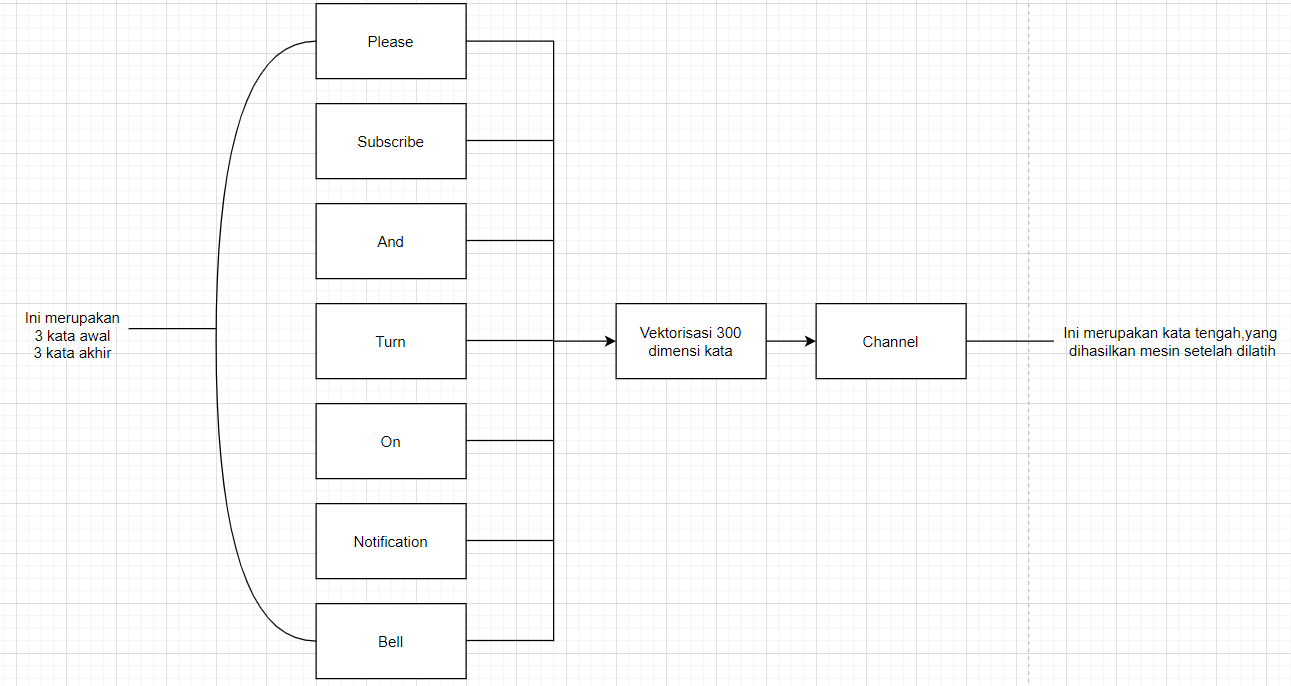
\includegraphics[width=12cm]{figures/1174084/5/teori3.png}
    \centering
    \caption{Teori 3}
\end{figure}

\item Jelaskan konsep vektorisasi untuk dokumen.dilengkapi dengan ilustrasi atau gambar.
\hfill\\
	Vektorisasi untuk dokumen hampir sama seperti vektorisasi untuk kata hanya saja pemilihan kata utama atau kata tengah terdapat pada satu dokumen jadi mesin akan membuat dimensi vektor 300 untuk dokumen dan nanti kata tengahnya akan di sandingkan pada dokumen yany terdapat pada dokumen tersebut.	
\begin{figure}[H]
    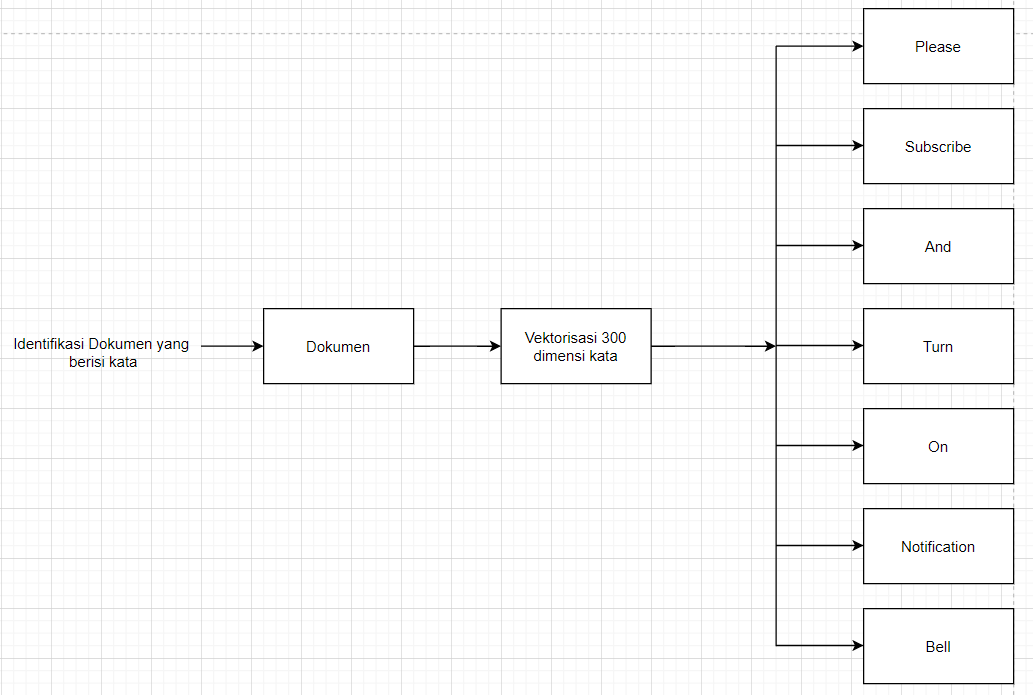
\includegraphics[width=8cm]{figures/1174084/5/teori4.png}
    \centering
    \caption{Teori 4}
\end{figure}

\item Jelaskan apa mean dan standar deviasi,dilengkapi dengan ilustrasi atau gambar.
	\hfill\\
mean merupakan petunjuk terhadap kata-kata yang di olah jika kata kata itu akurasinya tinggi berarti kata tersebut sering muncul begitu juga sebaliknya, sedangkan setandar defiation merupakan standar untuk menimbang kesalahan. sehingga kesalahan tersebut di anggap wajar misarkan kita memperkirakan kedalaman dari dataset merupakan 2 atau 3 tapi pada kenyataanya merupakan 5 itu merupakan kesalahan tapi masih bisa dianggap wajar karna masih mendekati perkiraan awal.
contoh pada gambar dibawah ini:
\begin{figure}[H]
    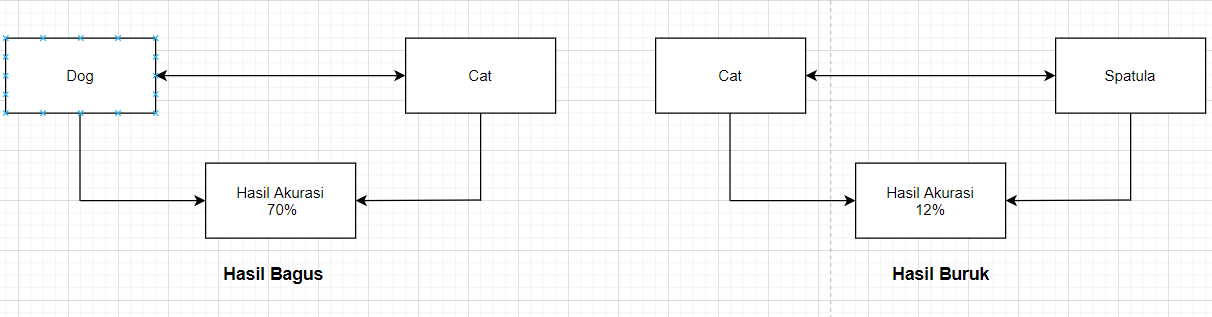
\includegraphics[width=8cm]{figures/1174084/5/teori5.png}
    \centering
    \caption{Teori 5}
\end{figure}

\item Jelaskan apa itu skip-gram,dilengkapi dengan ilustrasi atau gambar
	\hfill\\
	Skip-Gram adalah kebalikan dari konsep vektorisasi untuk kata dimana kata tengah menjadi acuan terhadap kata kata pelengkap dalam suatu kalimat.
\begin{figure}[H]
    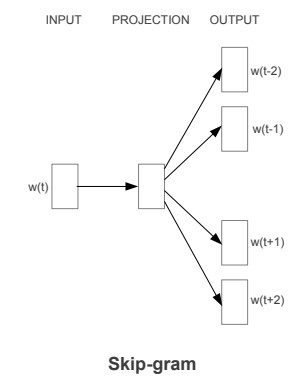
\includegraphics[width=8cm]{figures/1174084/5/teori6.png}
    \centering
    \caption{Teori 6}
\end{figure}
\end{enumerate}


\subsection{Praktek}
\begin{enumerate}


\item  mencoba dataset google dan penjelasan vektor dari kata love, faith, fall, sick, clear, shine, bag, car, wash, motor, dan cycle.
	\hfill\\
\begin{itemize}
\item berikut merupakan code import gensim digunakan untuk membuat data model atau rangcangan data yang akan di buat. selanjutnya dibuat variabel genmod yang berisi data vektor negativ. selanjutnya data tersebut di load agar data tersebut dapat di tampilkan dan di olah.	
	
\begin{figure}[H]
    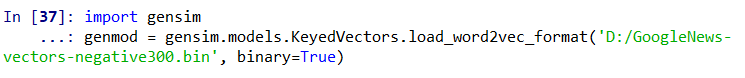
\includegraphics[width=8cm]{figures/1174084/5/1.png}
    \centering
    \caption{Praktek 1}
\end{figure}

\item berikut merupakan hasil lpengolahan kata love pada data google yang di load tadi. Sehingga memunculkan hasil vektor 300 dimensi untuk kata tersebut.

\begin{figure}[H]
    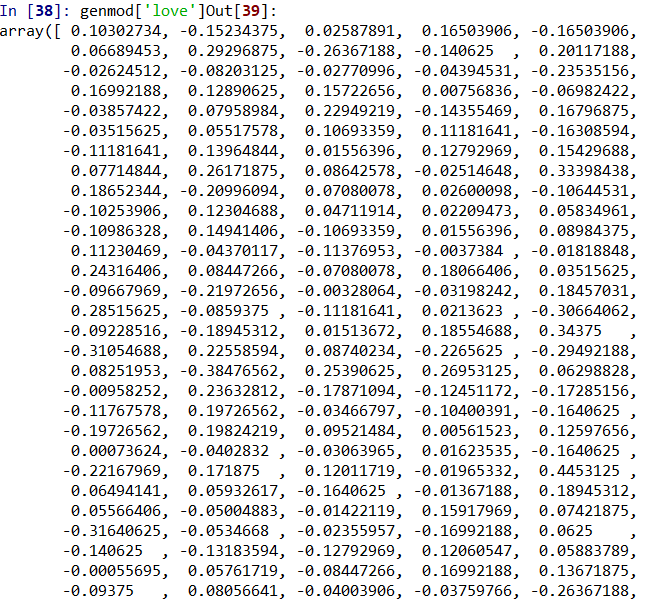
\includegraphics[width=8cm]{figures/1174084/5/2.png}
    \centering
    \caption{Praktek 1}
\end{figure}

\item berikut merupakan hasil lpengolahan kata faith pada data google yang di load. Sehingga memunculkan hasil vektor 300 dimensi untuk kata tersebut.

\begin{figure}[H]
    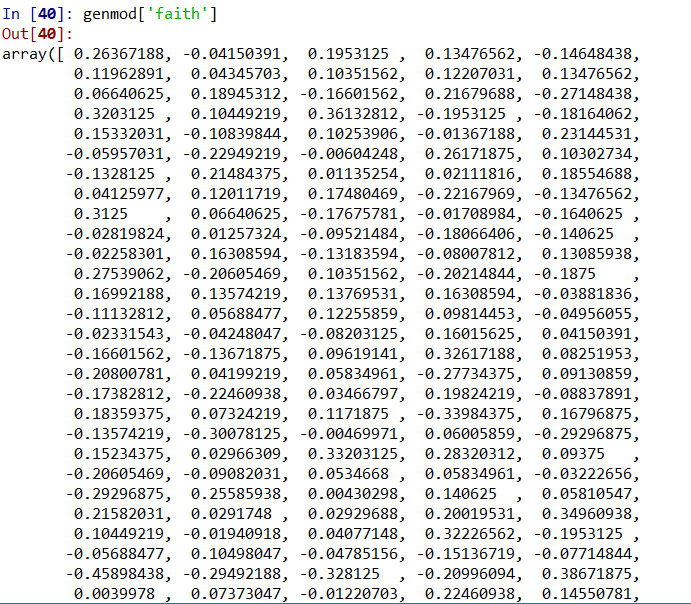
\includegraphics[width=8cm]{figures/1174084/5/3.png}
    \centering
    \caption{Praktek 1}
\end{figure}

\item berikut merupakan hasil lpengolahan kata fall pada data google yang di load. Sehingga memunculkan hasil vektor 300 dimensi untuk kata tersebut.

\begin{figure}[H]
    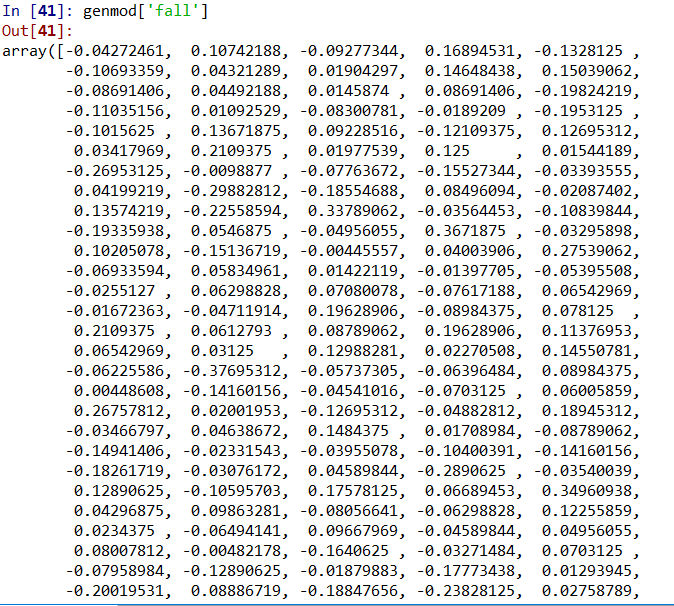
\includegraphics[width=8cm]{figures/1174084/5/4.png}
    \centering
    \caption{Praktek 1}
\end{figure}

\item berikut merupakan hasil lpengolahan kata sick pada data google yang di load. Sehingga memunculkan hasil vektor 300 dimensi untuk kata tersebut.

\begin{figure}[H]
    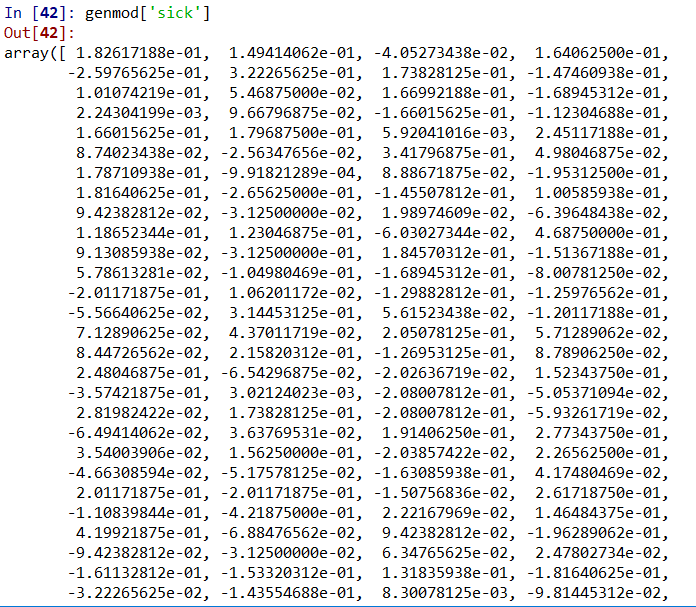
\includegraphics[width=8cm]{figures/1174084/5/5.png}
    \centering
    \caption{Praktek 1}
\end{figure}

\item berikut merupakan hasil lpengolahan kata clear pada data google yang di load. Sehingga memunculkan hasil vektor 300 dimensi untuk kata tersebut.

\begin{figure}[H]
    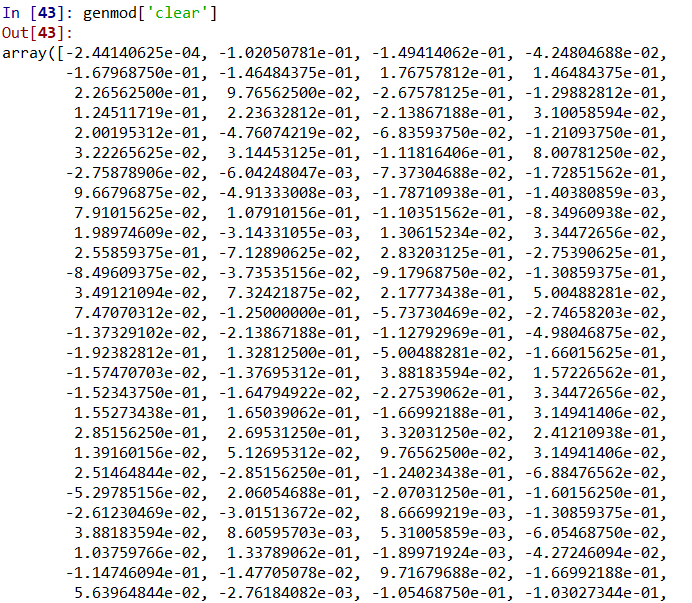
\includegraphics[width=8cm]{figures/1174084/5/6.png}
    \centering
    \caption{Praktek 1}
\end{figure}

\item berikut merupakan hasil lpengolahan kata shine pada data google yang di load. Sehingga memunculkan hasil vektor 300 dimensi untuk kata tersebut. 

\begin{figure}[H]
    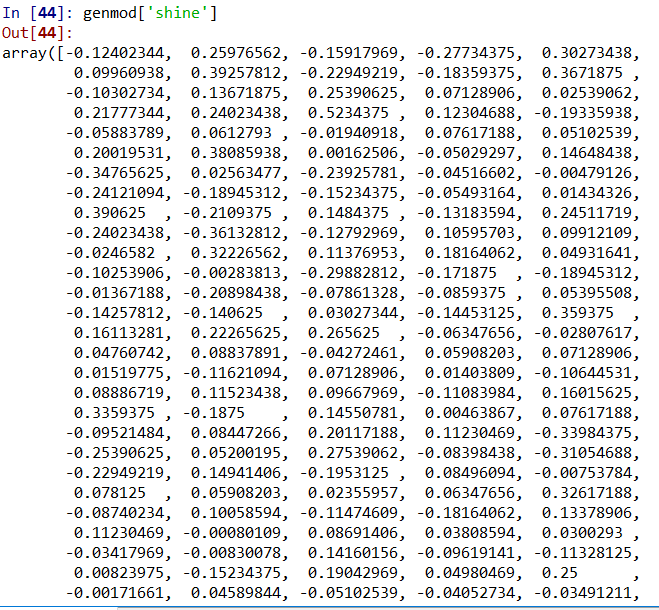
\includegraphics[width=8cm]{figures/1174084/5/7.png}
    \centering
    \caption{Praktek 1}
\end{figure}

\item berikut merupakan hasil lpengolahan kata bag pada data google yang di load. Sehingga memunculkan hasil vektor 300 dimensi untuk kata tersebut.

\begin{figure}[H]
    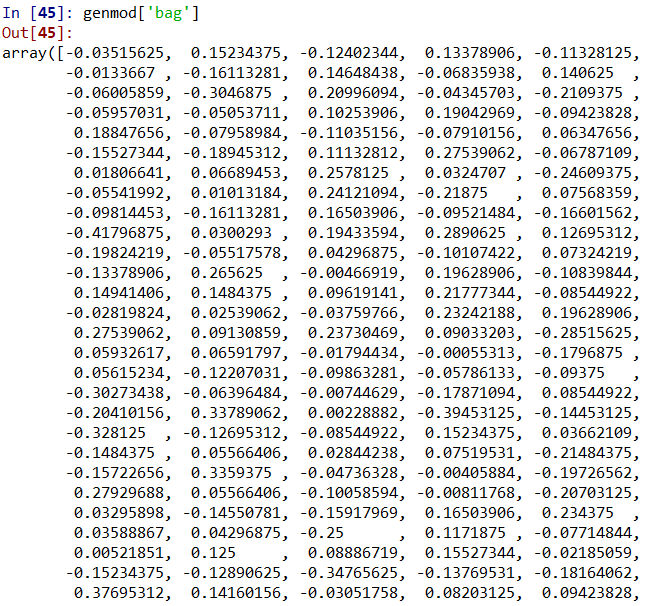
\includegraphics[width=8cm]{figures/1174084/5/8.png}
    \centering
    \caption{Praktek 1}
\end{figure}

\item berikut merupakan hasil lpengolahan kata car pada data google yang di load. Sehingga memunculkan hasil vektor 300 dimensi untuk kata tersebut.

\begin{figure}[H]
    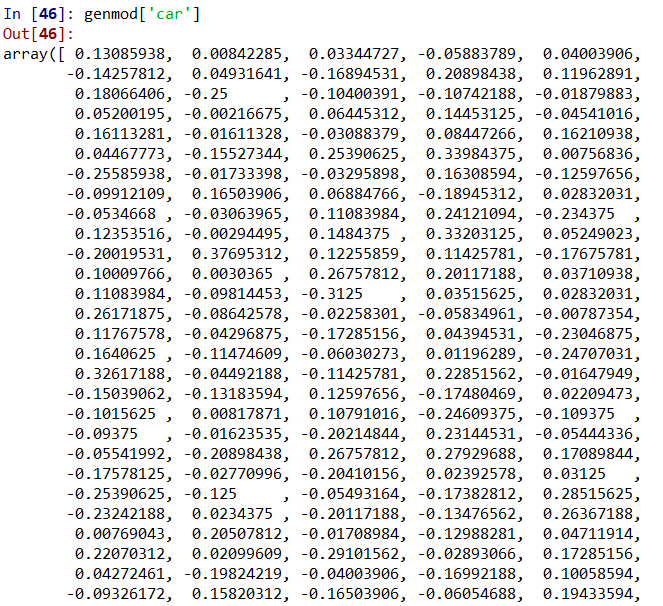
\includegraphics[width=8cm]{figures/1174084/5/9.png}
    \centering
    \caption{Praktek 1}
\end{figure}

\item berikut merupakan hasil lpengolahan kata wash pada data google yang di load. Sehingga memunculkan hasil vektor 300 dimensi untuk kata tersebut.

\begin{figure}[H]
    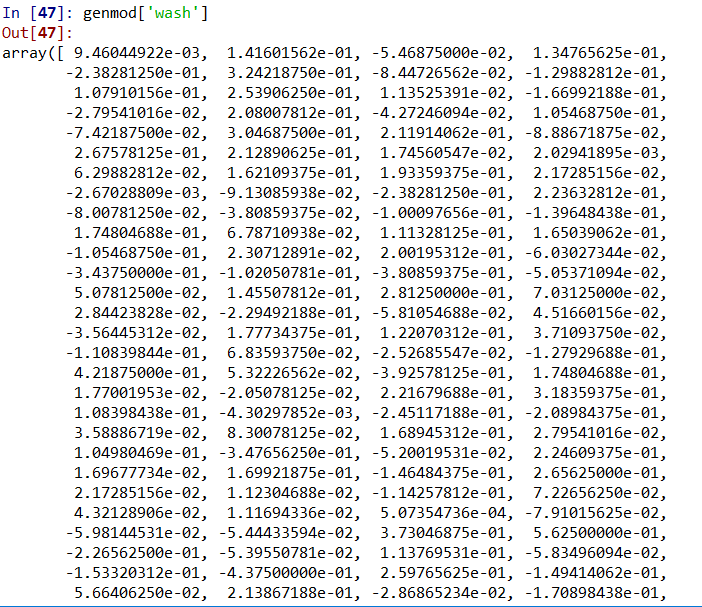
\includegraphics[width=8cm]{figures/1174084/5/10.png}
    \centering
    \caption{Praktek 1}
\end{figure}

\item berikut merupakan hasil lpengolahan kata motor pada data google yang di load. Sehingga memunculkan hasil vektor 300 dimensi untuk kata tersebut.

\begin{figure}[H]
    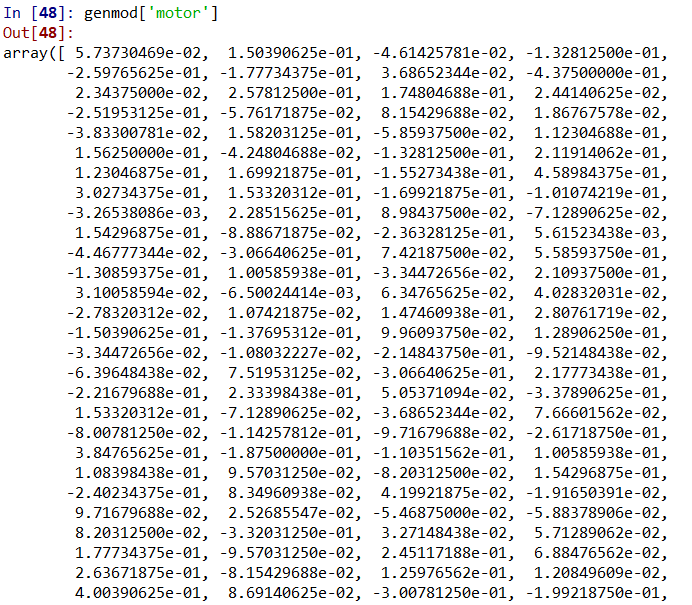
\includegraphics[width=8cm]{figures/1174084/5/11.png}
    \centering
    \caption{Praktek 1}
\end{figure}

\item berikut merupakan hasil lpengolahan kata cycle pada data google yang di load. Sehingga memunculkan hasil vektor 300 dimensi untuk kata tersebut.

\begin{figure}[H]
    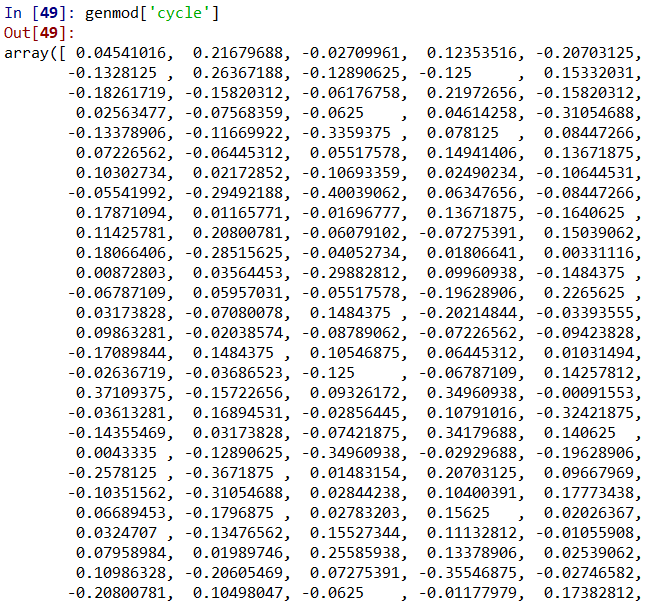
\includegraphics[width=8cm]{figures/1174084/5/12.png}
    \centering
    \caption{Praktek 1}
\end{figure}

\item berikut merupakan hasil dari similaritas kata kata yang di olah menjadi matrix tadi adapun persentase untuk perbandingan setiap katanya yaitu 9 persen untuk kata wash dan clear 7 persen untuk kata bag dan love 48 persen untuk kata motor dan car 12 persen untuk kata sick dan faith dan terakhir yaitu 6 persen untuk kata cycle dan shine.

\begin{figure}[H]
    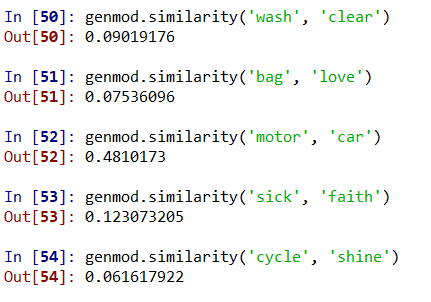
\includegraphics[width=8cm]{figures/1174084/5/13.png}
    \centering
    \caption{Praktek 1}
\end{figure}
\end{itemize}


\item  jelaskan dengan kata dan ilustrasi fungsi dari extract words dan PermuteSentences
	\hfill\\
pada code berikut merupakan hasil dari running code untu ekstrak word dimana pada baris ke tiga dimasukan perintah untuk menghapus tag html yang terdapat dalam file tesebut selanjutnya pada baris ke 4 yaitu perintah untuk menghilangkan tanda kutip satu selanjutnya pada baris ke 5 yaitu perintah untuk menghapus tanda baca pada file tersebut dan yang terakhir yaitu perintah untuk menghapus dable sepasi atau sepasi berurutan. setelah itu dibuat clas bari dari random yang bertujuan untuk mengkocok data yang ada pada file tersebut kemudian class permute sentence tersebut akan di gunkan untuk mengolah data selanjutnya. untuk lebih jelasnya dapat dilihat pada gambar	

\begin{figure}[H]
    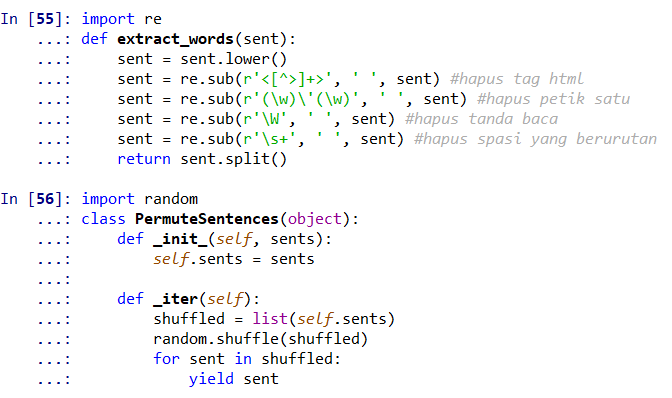
\includegraphics[width=8cm]{figures/1174084/5/14.png}
    \centering
    \caption{Praktek 2}
\end{figure}

\item Jelaskan fungsi dari librari gensim TaggedDocument dan Doc2Vec disertai praktek pemakaiannya
	\hfill\\
	gensim merupakan library untuk memodelkan topik unsuperpise atau memodelkan bahasa dengan model unsuperpise. Sadangkan taget dokumen digunakan untuk TaggetDokumen berarti memasukan dokumen untuk di olah oleh mesin. Kemudian Doc2Vect dugunakan untuk membandingkan dokumen apakah isi dari dokumen itu bobotnya sama dengan dokumen yang disandingkan. menunjukan di baris ke satu dilakukan dari library gensim dokumen mengimport method TaggedDocument lalu pada baris kedua dari library gensim model melakukan import metod Doc2Vec.
\begin{figure}[H]
    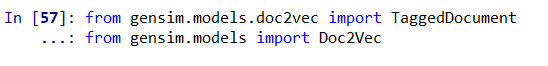
\includegraphics[width=8cm]{figures/1174084/5/15.png}
    \centering
    \caption{Praktek 3}
\end{figure}

\item Jelaskan dengan kata dan praktek cara menambahkan data training dari file yang dimasukkan kepada variabel dalam rangka melatih model doc2vac
	\hfill\\
	cara memasukan data traning file pertama tentukan terlebih dahulu tempat file dokumen tersebut disimpan kemudian import librari os setelah itu buat variabel unsup\_sentences yang berisikan array kosong, lalu tentukan file yang akan dimasukan setelah itu lakukan os listdir pada data yang akan dimasukan kemudian semua data tersebut di inisialisasi menjadi f kemudian nama f tersebut dimasukan ke variabel unsup. pada codingan tersebut merupakan praktikum untuk memasukan data doc2vec
\begin{figure}[H]
    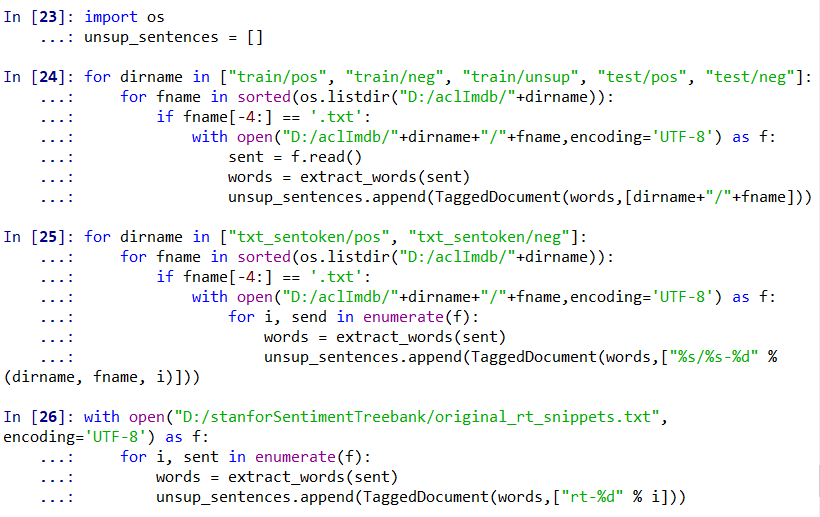
\includegraphics[width=8cm]{figures/1174084/5/16.png}
    \centering
    \caption{Praktek 4}
\end{figure}

\item Jelaskan dengan kata dan praktek kenapa harus dilakukan pengocokan dan pembersihan data
	\hfill\\
hal ini harus dilakukan supaya data lebis gambang untuk di olah dan meningkatkan tingkat akurasi dari proses pengolahan data Doc2Vec. kemudian harus dilakukan pembersihan data agar memori pc atau laptop yang di gunakan untuk mengolah data menjadi ringan dan menambah peforma dari mesin itu sendiri untuk codingan pertama lakukan terlebih dahulu rendomisasi. selanjutnya membuat variabel baru dengan nama mute yang di isi data class random dan data unsup\_sentence. kemudian setelah pengolahan data dilakukan pembersihan dengan melakukan code.	

\begin{figure}[H]
    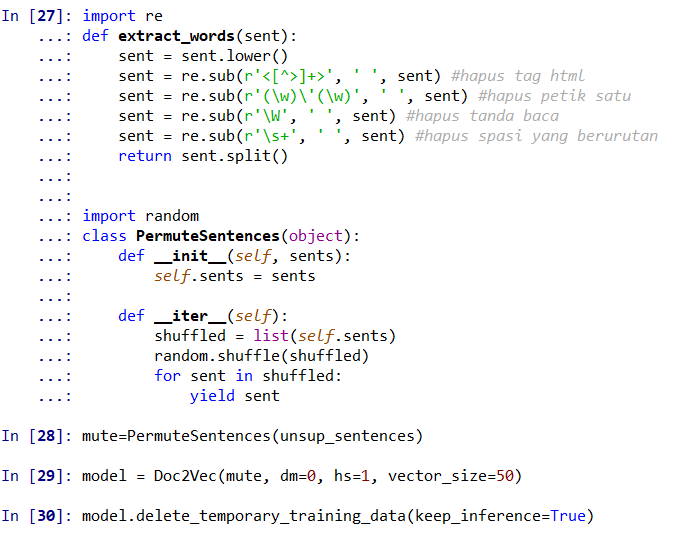
\includegraphics[width=8cm]{figures/1174084/5/17.png}
    \centering
    \caption{Praktek 5}
\end{figure}

\item Jelaskan dengan kata dan praktek kenapa model harus di save dan kenapa temporari training harus dihapus
	\hfill\\
	suapaya dalam pengolahan data tidak perlu menjalankan kembali data vektorisasi serta untuk meringankan beban ram. kemudian temporary harus dihapus guna meningkatkan peforma komputer.

\begin{figure}[H]
    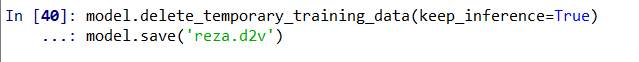
\includegraphics[width=12cm]{figures/1174084/5/18.png}
    \centering
    \caption{Praktek 6}
\end{figure}

\item jalankan dengan kta dan praktek maksud dari infer code
	\hfill\\
	inver\_code digunakan untuk membandingkan data doc2vec yang telah di olah dengan kata yang baru atau data yang ada dalam perintah vector itu sendiri contoh membandingkan kata (i will go home) untuk lebih jelasnya dapat di lihat pada gambar. kemudian untuk hasil running code tersebut dapat di lihat pada gambar pada hasil gambar tersebut terdapat hasil vektor yang rata rata berada pada kisaran 0,2 an yang berarti kata yang dimasukan pada inter\_vec datanya ada pada doc2vec atau ada data yang bobotnya menyamai kata-kata di dalam dokumen tersebut.
\begin{figure}[H]
    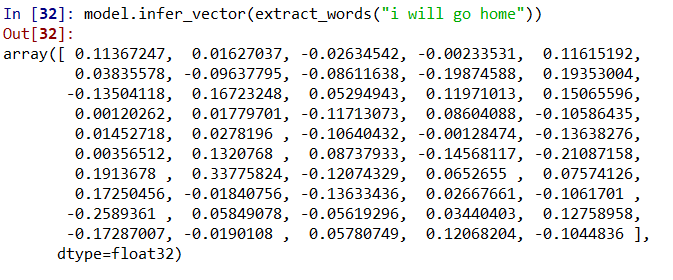
\includegraphics[width=8cm]{figures/1174084/5/19.png}
    \centering
    \caption{Praktek 7}
\end{figure}

\item  Jelaskan dengan praktek dan kata maksud dari cosine similarity
	\hfill\\
	consine\_simirarity setelah melakukan pengolahan data doc2vec dilakukan consine simirarity yang bertujuan untuk membandingkan data dengan yang telah di olah tadi apakah hasilnya mirip atau tidak untuk caranya yaitu dengan cara mencoba codingan yang terdapat pada gambar berikut maka akan muncul hasilnya berapa persen dengan tulisan 0.03 sekian yang berarti tingkat kemiripan dokumen yang kita uji tadi, untuk hasilnya dapat dilihat pada gambar berikut.
	
\begin{figure}[H]
    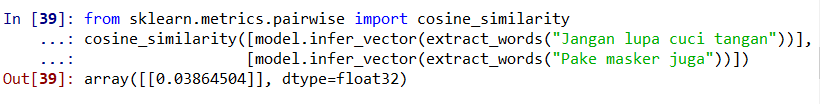
\includegraphics[width=8cm]{figures/1174084/5/20.png}
    \centering
    \caption{Praktek 8}
\end{figure}

\item  Jelaskan dengan praktek score dari cross validation
	\hfill\\
	Melakukan perhitungan presentase dengan menggunakan cross\_validation dengan metode kneighborsClassifier. Menggunakan dataset iris
	\begin{figure}[H]
    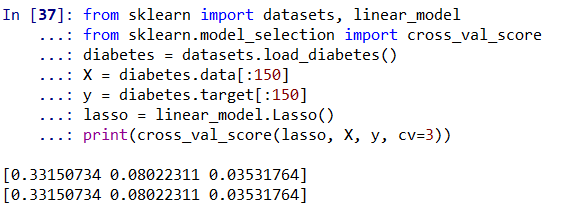
\includegraphics[width=8cm]{figures/1174084/5/21.png}
    \centering
    \caption{Praktek 9}
\end{figure}
\end{enumerate}

\subsection{Penanganan Error}
\begin{enumerate}
	\item FileNotFound Error
	\hfill\break
		\begin{figure}[H]
			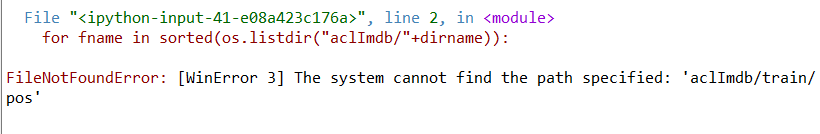
\includegraphics[width=7cm]{figures/1174084/5/error.png}
			\centering
			\caption{FileNotFound Error}
		\end{figure}
	\item Jenis error
	\begin{itemize}
		\item FileNotFound Error
	\end{itemize}
	\item Cara Penanganan
	\hfill\break
	Menyesuaikan tempat/direktori file berada
\end{enumerate}

\subsection{Bukti Tidak Plagiat}
\begin{figure}[H]
	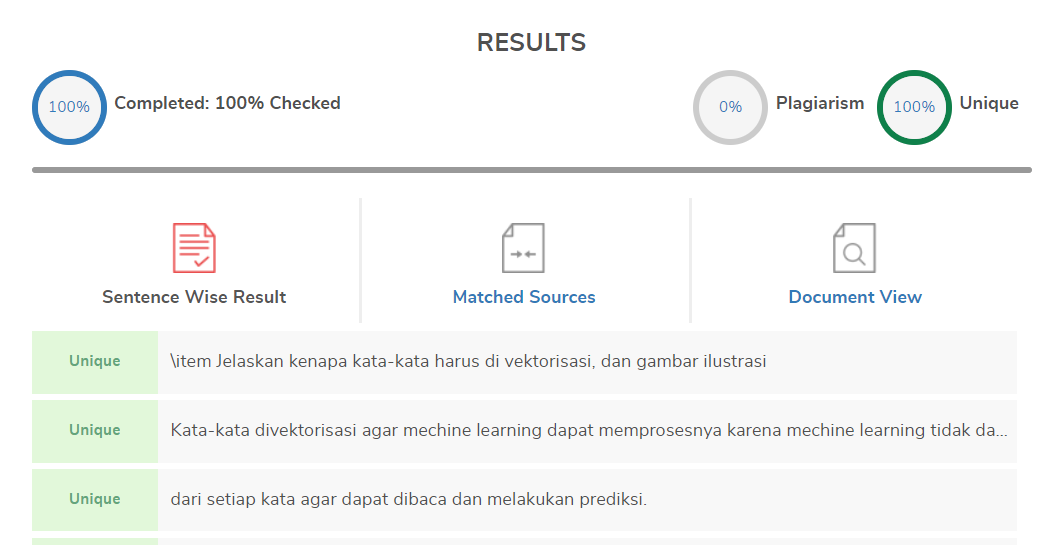
\includegraphics[width=4cm]{figures/1174084/5/plagiarism.png}
	\centering
	\caption{plagiarism}
\end{figure}


\subsection{Link Video Youtube}
https://youtu.be/0hiPlSo83jY

